\documentclass[11pt]{scrartcl}
\usepackage[utf8]{inputenc} % Kodierung der Textdatei mit Sonderzeichen
\usepackage[ngerman]{babel} % Sprache fuer Inhaltsverzeichnis etc.
\usepackage{amssymb} % Mathematische Symbole
\usepackage{amsmath} % Mehr mathematische Konstrukte
\usepackage{graphicx} % Um Bilder einbinden zu koennen
\usepackage{float} % fuer \begin{figure}[H]
\usepackage{icomma} % laesst das Komma als Dezimaltrennzeichen interpretieren
\usepackage{fix-cm} % für die große Titelschrift
\usepackage[pdftex]{hyperref} % Hyperlinks im Dokument
\hypersetup{colorlinks=true, linkcolor=black, citecolor=black, filecolor=black, urlcolor=black, pdftitle={MHD-Generator - Projektpraktikum 09/10 Gruppe 5}}


\newcommand{\unit}[1]{\ensuremath{\,\mathrm{#1}}} % Einheiten schreiben sich immer aufrecht!
\newcommand{\degr}{\ensuremath{^\circ}}
\newcommand{\cel}{\ensuremath{\degr\mathrm{C}}}
\newcommand{\dif}{\ensuremath{\mathrm{d}}}
\newcommand{\pdif}[2]{\ensuremath{\frac{\partial#1}{\partial#2}}}
\newcommand{\ee}[1]{\ensuremath{\cdot\! 10^{#1}}}
\newcommand{\abb}[1]{\hyperref[#1]{Abb.~\ref{#1}}}
\newcommand{\tab}[1]{\hyperref[#1]{Tabelle~\ref{#1}}}

\setlength{\parindent}{1em}
\setlength{\parskip}{0.5\baselineskip}


\title{MHD-Generator - Gruppe 5 WS 09/10, Projektpraktikum der Uni Erlangen}
\date{09.11.2009 -- 04.12.2009}
\author{Michele Collodo, Andreas Glossner, Karl-Christoph G\"odel, Bastian Hacker, Maria Obst, Alexander Wagner, David Winnekens}



\begin{document}
\sloppy % laesst Latex nicht ueber den Rand rausschreiben
\thispagestyle{empty}
\large{Projektpraktikum WS 09/10}
\hfill
\raisebox{-1.4cm}{
\includegraphics[width=5cm]{images/fau.pdf}}
\\begin{equation}8\baselineskip]
\begin{center}
{\fontsize{36}{54}\textbf{MHD-Generator}}
\\begin{equation}2\baselineskip]
{\Large 09.11.2009 -- 04.12.2009}
\\begin{equation}7\baselineskip]
{\huge\textbf{PPG 5}}\\begin{equation}0.5\baselineskip]
{\large\textbf{
Michele Collodo,
Andreas Glossner,\\
Karl-Christoph G\"odel,
Bastian Hacker,\\
Maria Obst,
Alexander Wagner,
David Winnekens}\\
Tutor: Xiaoyue Jin}
\vfill



\small{\url{http://pp.physik.uni-erlangen.de/groups/ws0910/ppg5/ppg5\_start.html}}
\end{center}
\newpage



\tableofcontents
\vfill



\begin{abstract}
Der magnetohydrodynamische (MHD) Generator wandelt die Bewegungsenergie von Teilchen in elektrische Leistung um. Ziel des Projekts war es, diesen Effekt an einer selbst gebauten Zelle mit strömendem Salzwasser nachzuweisen. Hierzu wurde mit Hilfe von vier Spulen ein Magnetfeld von $160 \unit{mT}$ erzeugt und die durch den Effekt entstandene Spannugn an zwei längsseitig angebrachten Elektroden abgenommen. Die theoretischen Zusammenhänge haben sich dabei alle experimentell sehr gut nachweisen lassen, die Spannungswerte an der Zelle waren jedoch vergleichsweise niedrig. Zur praktischen Einsetzbarkeit müsste noch die Leitfähigkeit des Fluids gesteigert werden.
\end{abstract}
\newpage
%%%%%%%%%%%%%%%%%%%%%%%%%%%%%%%%%%%%%%%%%%%%%%%%%%
%Das Plexiglasteil wird im Folgenden: "Zelle" genannt
%%%%%%%%%%%%%%%%%%%%%%%%%%%%%%%%%%%%%%%%%%%%%%%%%%


\section{Einleitung}	%% maria: ist fertig, kommentare, wuensche, anregungen?
Die Frage der Energieerzeugung hat in der Physik der letzten Jahrhunderte immer eine bedeutende Rolle gespielt. Eine vielversprechende M\"oglichkeit schien das Ausnutzen von magnetischen Feldern. Die ersten \"Uberlegungen zum Magnetohydrodynamischen Generator, kurz MHD-Generator, machte Michael Faraday schon 1832. Er führte Experimente an der Waterloo Bridge in London durch und entdeckte den zugrunde liegenden Effekt des MHD-Generators, indem er Spannung maß, die vom Fluß der Themse im Erdmagnetfeld erzeugt wurde.
140 Jahre später wurde mit einer Leistung von 25MW der bisher größte MHD-Generator in der Sowjetunion fertiggestellt und ans Moskauer Stromnetz angeschlossen. Zur Zeit gibt es die Aussicht, diesen Effekt in Kern- oder Fusionskraftwerken zu nutzen, in welchen flüssiges Metall als Fluid genutzt werden soll.

\section{Theorie}	%% maria

%%% mir faellt nix mehr ein, was koennt ich da noch reinschreiben?

Das Prinzip des MHD-Generators beruht auf der Lorentzkraft,
\begin{equation}
\vec{F} = q \cdot \left(\vec{v} \times \vec{B} \right),
\end{equation}
die in einem Magnetfeld auf eine bewegte Ladung wirkt. Wird also eine leitende Fl\"ussigkeit durch ein m\"oglichst homogenes, starkes Magnetfeld geschickt, welches senkrecht zur Flussrichtung gerichtet ist, werden positive und negative Ladungen entsprechend der Rechten-Hand-Regel in entgegengesetzte Richtungen abgelenkt. Bringt man dann in jeder dieser Richtungen je eine Elektrode an, kann man eine Spannung abgreifen und hat so eine Generatorzelle konstruiert. Die hierbei entstehende Spannung ist
\begin{equation}
U = B \cdot v \cdot d,
\end{equation}
wobei $d$ den Abstand zwischen den beiden Elektroden und $v$ die Flie\ss{}geschwindigkeit der Fl\"ussigkeit bezeichnet. Der gemessene Strom ist dann 
\begin{equation}
I = v \cdot B \cdot A \cdot \sigma,
\end{equation}
wo $A$ die Fl\"ache einer Elektrode und $\sigma$ die Leitf\"ahigkeit der Fl\"ussigkeit ist. Daraus ergibt sich eine Leistung des Generators von
\begin{equation}
P = U \cdot I = B^{2} \cdot v^{2} \cdot A \cdot d \cdot \sigma.
\end{equation}


\section{Konstruktion und Aufbau}

\subsection{Konstruktion des Magnetfelds}		%%andi
<<<<<<< HEAD:exp2/protokoll/mhd-generator.tex
Im Vorfeld der eigentlichen Messungen an der Zelle wurde eine möglichst optimale Konstruktion des Magnetfelds ermittelt. Ziel war es, bei einer Feldstärke von rund $0,1 \unit{T}$ ein möglichst im gesamten Bereich der Zelle homogenes Feld zu erhalten.

Zunächst wurden verschiedene Permanentmagneten eingesetzt, die jedoch allesamt unbefriedigende Ergebnisse lieferten. Die eingesetzten Stabmagneten erzielten eine maximale Feldstärke von $0,07 \unit{T}$, das der zur Verfügung stehenden Hufeisenmagneten war noch wesentlich niedriger. Die größte Feldstärke wurde an Ringpermanentmagneten ($B\approx0,3T$) gemessen; dieser Wert fiel jedoch schon im Abstand von wenigen $\unit{mm}$ stark ab ($1/r^3$-Abhängigkeit !) und war deshalb ebenfalls ungeeignet.
=======
Im Vorfeld der eigentlichen Messungen an der Zelle wurde die möglichst optimale Konstruktion des Magnetfelds ermittelt. Ziel war es, bei einer Feldstärke von rund $0,1 T$, ein möglichst im gesamten Bereich der Zelle homogenes Feld zu erhalten.

Zunächst wurden verschiedene Permanentmagneten eingesetzt, die jedoch allesamt unbefriedigende Ergebnisse lieferten. Die eingesetzten Stabmagneten erzielten eine maximale Feldstärke von $0,07T$, die der zur Verfügung stehenden Hufeisenmagneten war noch wesentlich niedriger. Die größte Feldstärke wurde an Ringpermanentmagneten ($B\approx0,3T$) gemessen; dieser Wert fiel jedoch schon im Abstand von wenigen $mm$ stark ab ($1/r^3$-Abhängigkeit) und war deshalb ebenfalls ungeeignet.
>>>>>>> 0dfd7a8e82e906a49ac84748d4abd0738047c329:exp2/protokoll/mhd-generator.tex

Folglich wurde ein Aufbau mit Elektromagneten gewählt. Zum Einsatz kamen dabei vier Spulen mit je 1000 Windungen (Anordnung siehe \abb{bfeld-vor2}).

\begin{figure}[ht]
\begin{center}
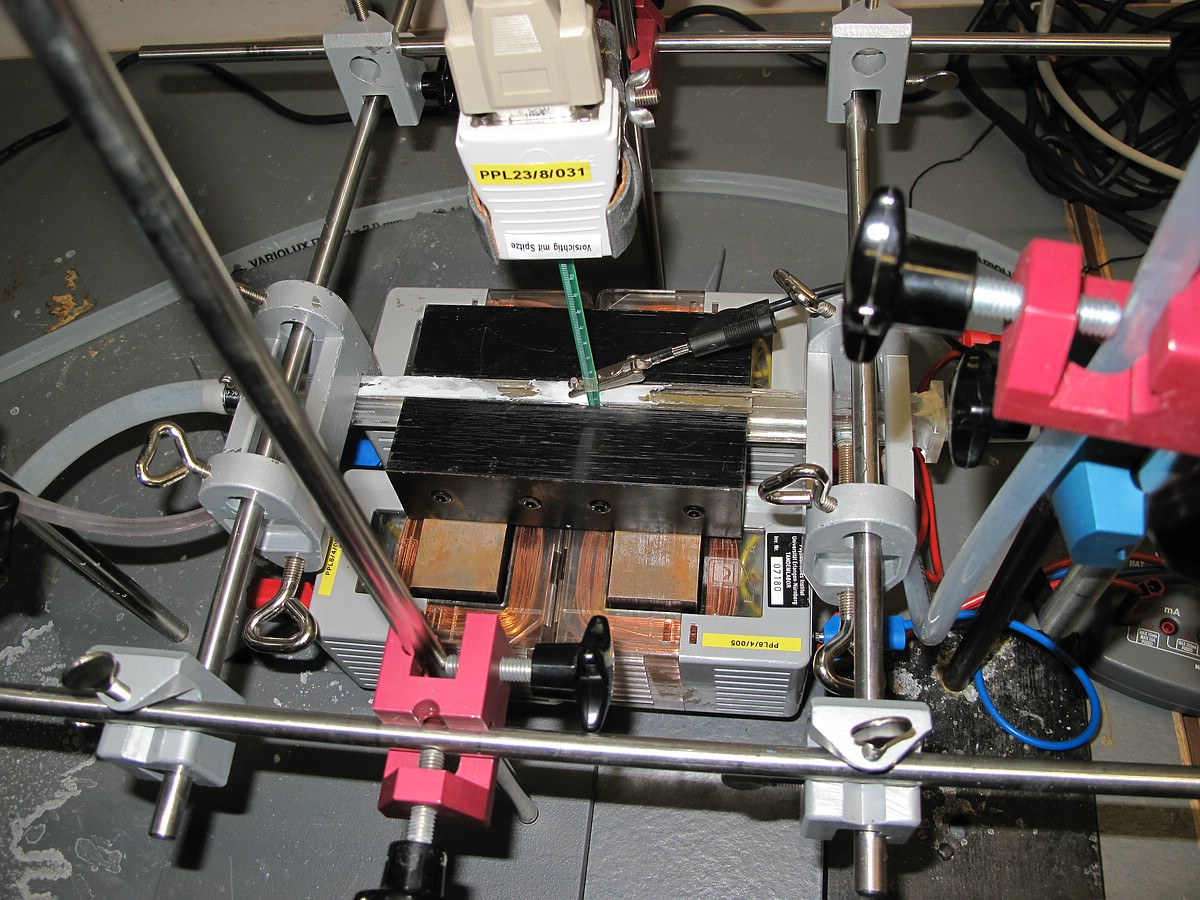
\includegraphics[width=0.8\textwidth]{images/bfeld-vor2.jpg}
\end{center}
\vspace{-1.5\baselineskip}
\caption{Anordnung der vier Spulen zum Erzeugen des Magnetfelds}
\label{bfeld-vor2}
\end{figure}

<<<<<<< HEAD:exp2/protokoll/mhd-generator.tex
Zunächst wurde eine kurze Messung zur Ermittlung der Abhängigkeit der Magnetfeldstärke vom Abstand zwischen den beiden Eisenjochen durchgeführt. Zu erwarten war wegen 
\begin{equation*}
B = \frac{\mu \cdot \mu_{0} \cdot N \cdot I}{\mu \cdot d + 2 \pi \cdot R}
\end{equation*}
=======
Zunächst wurde eine kurze Messung zur Ermittlung der Abhängigkeit der Magnetfeldstärke vom Abstand zwischen den beiden Eisenjochen
%% wie heissen die dinger schnell wieder
durchgeführt. Zu erwarten war wegen 
\begin{equation}
B = \frac{\mu \cdot \mu_{0} \cdot N \cdot I}{\mu \cdot d + 2 \pi \cdot R}
\end{equation}
>>>>>>> 0dfd7a8e82e906a49ac84748d4abd0738047c329:exp2/protokoll/mhd-generator.tex
in etwa eine $1/d$-Abhängigkeit, wobei $\mu$ die Materialkonstante des Eisens, $N$ die Windungszahl, $d$ der Abstand zwischen den beiden Eisenjochen und $R$ der Radius der "`Gesamtspule"' ist. Die "`Gesamtspule"' ist dabei die gesamte Anordnung der vier Einzelspulen und kann in erster Näherung als kreisförmig angenommen werden.

Wie in \abb{bfeld-vor2} gut sichtbar, hat sich diese Annahme zumindest qualitativ bestätigt. Bei der angelegten Spannung von $1 \unit{A}$ und einem Radius der Gesamtanordnung von $8.5 \unit{cm}$ ergibt sich für $N=2992$ die eingezeichnete Fitkurve. Der $N$-Wert weicht zwar deutlich von den tatsächlichen 1000 Wicklungen ab. Dies dürfte jedoch auf die von einer idealen kreisförmig Geometrie abweichende Anordnung sowie die recht ungenauen Messwerte zurückzuführen sein.

In Folge der vorliegenden Messergebnisse wurde der Abstand zwischen den beiden Eisenjochen beim eigentlichen Versuch dann möglichst klein gewählt (auf $1.1 \unit{cm}$, das entspricht der Zellbreite).

\begin{figure}[ht]
\begin{center}
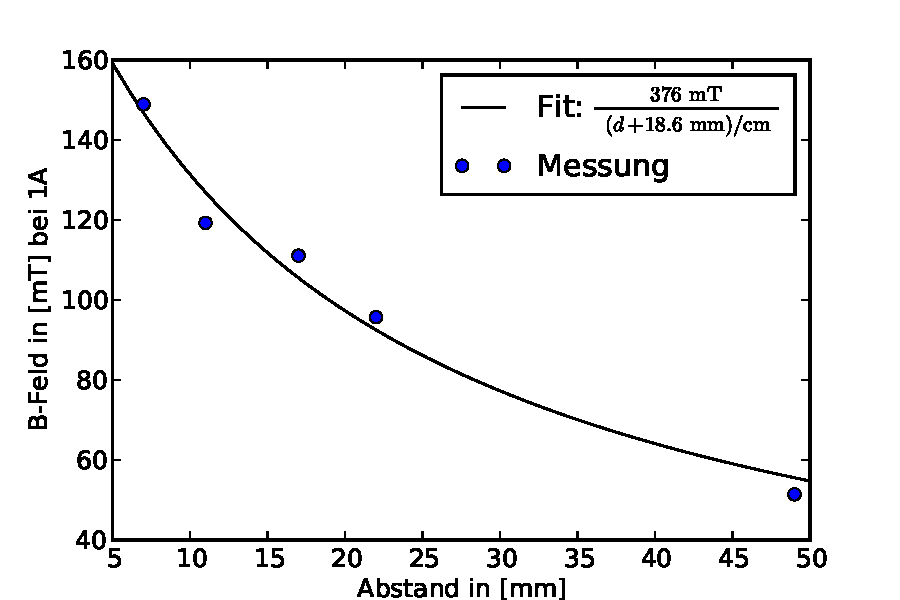
\includegraphics[width=0.8\textwidth]{images/messung_B-Feld-Abstand.pdf}
\end{center}
\vspace{-1.5\baselineskip}
\caption{Abhängigkeit der Magnetfeldstärke vom Abstand zwischen den beiden Eisenjochen (siehe \abb{bfeld-vor2})}
\label{messung_B-Feld-Abstand}
\end{figure}


\begin{figure}[ht]
\begin{center}
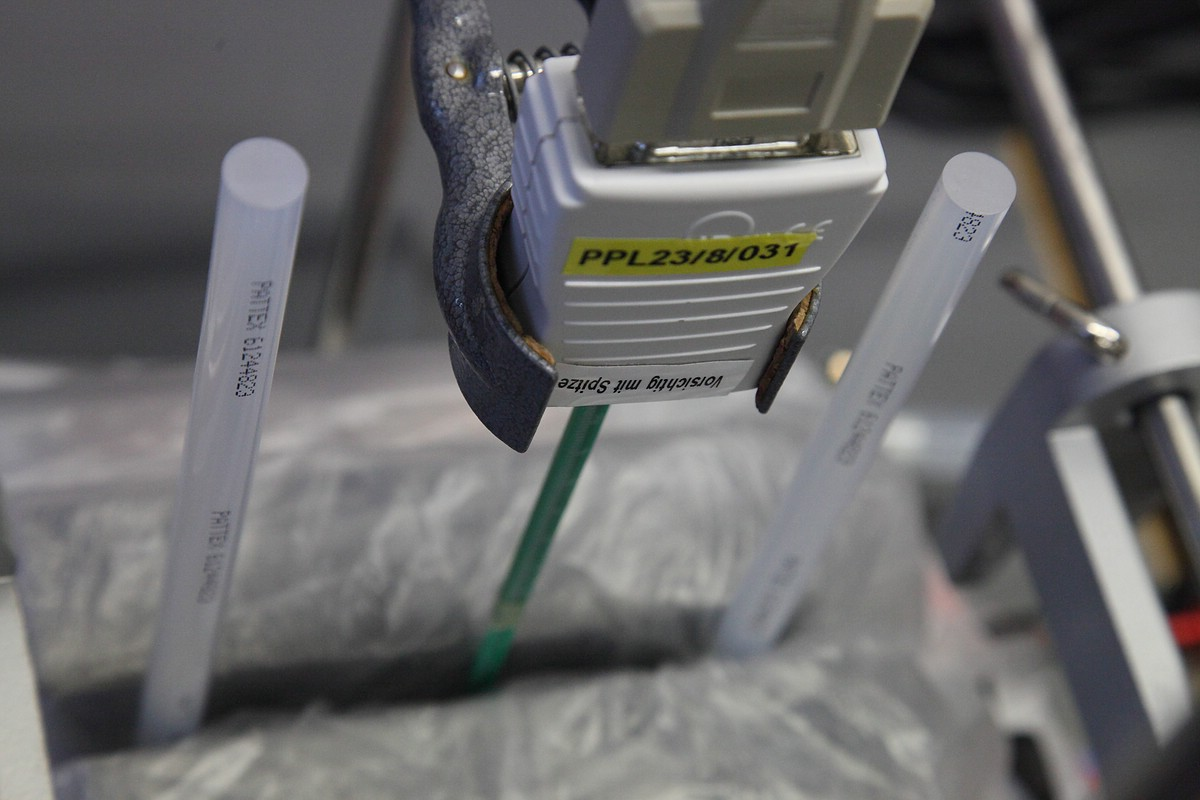
\includegraphics[width=0.8\textwidth]{images/bfeld-vor1.jpg}
\end{center}
\vspace{-1.5\baselineskip}
\caption{Vormessung ohne Zelle zur B-Feldst\"arke, die Plastikst\"abe dienen zum Einstellen verschiedener Spaltbreiten}
\label{bfeld-vor1}
\end{figure}


Um die Geometrie des Magnetfeldes zu ermitteln, wurde ein weiterer Versuch im Vorfeld durchgeführt. Dazu wurde die magnetische Feldstärke bei drei verschiedenen Abständen ($d_1=1.5 \unit{cm}, d_2=2.5 \unit{cm}, d_3=3.5 \unit{cm}$) jeweils an verschiedenen Punkten zwischen den beiden Eisenjochen gemessen. Die Messpunkte lagen dabei im homogenen Bereich des Magnetfeldes, durch den später auch das Salzwasser in der Zelle fließen sollte. Ausnahme waren zwei Messungen $1 \unit{cm}$ links und rechts des Eisenjochspaares sowie eine Messung im Abstand $2 \unit{cm}$ über dem Zentrum des homogenen Bereichs (d.h. knapp $1 \unit{cm}$ über den Eisenjochen).

Wie in \hyperref[vormessung_magnetfeld]{Abb.~\ref{vormessung_magnetfeld}} gut erkennbar, war das Magnetfeld bei allen drei Abständen im für die Zelle relevanten Bereich sehr homogen und damit gut geeignet für die weiteren Messungen. Außerdem zeigte sich, dass mit dem gewählten 4-Spulen-Aufbau bei einem Abstand von $d_1=1.5 \unit{cm}$ ein Magnetfeld von rund $82 \unit{mT}$ erreicht werden konnte, was für einen mit den gegebenen Möglichkeiten nachweisbaren Effekt völlig ausreichte.
Der relativ deutliche Abfall der Feldstärke schon knapp $1 \unit{cm}$ über den Eisenjochen auf rund $58 \unit{mT}$ konnte ignoriert werden, da sich die angefertigte Zelle bei allen folgenden Messungen vollständig im Bereich des homogenen Magnetfelds befand. 

\begin{figure}[ht]
\begin{center}
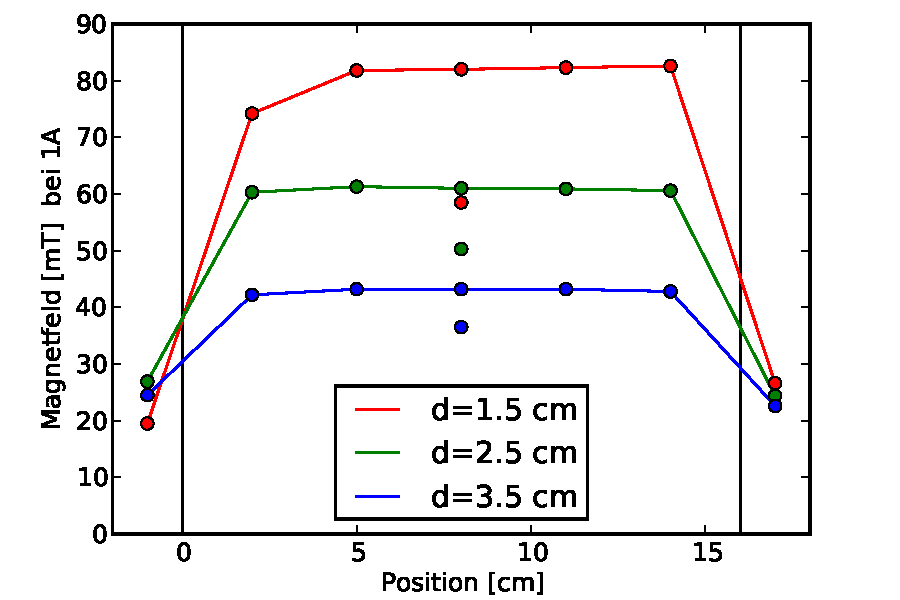
\includegraphics[width=0.8\textwidth]{images/vormessung_magnetfeld.pdf}
\end{center}
\vspace{-1.5\baselineskip}
\caption{Stärke des Magnetfeldes entlang der Achse (Messung mittig, einzelne Punkte am oberen Rand)}
\label{vormessung_magnetfeld}
\end{figure}

In einer letzten Vormessung wurde noch der Zusammenhang zwischen der an den Spulen angelegten Stromstärke und der Magnetfeldstärke ermittelt. Von den untersuchten Theorien passte dabei beim Ermitteln der Fitkurve am besten das arctan-Modell von Süß et al., Theoretische Grundlagen der Elektrotechnik 1 \footnote{Theoretische Grundlagen der Elektrotechnik 1; Süße, Burger, Diemar, Marx, Ströhla; S. 142 ff.}. Dabei ergab sich die in \hyperref[messung_Strom-B-Feld]{Abb.~\ref{messung_Strom-B-Feld}} erkennbare Fitkurve.

Gewählt wurde dabei ein Jochabstand von $1\unit{mm}$, was der Breite der verwendeten Hallsonde entspricht. Keine Rolle spielte erwartungsgemäß, ob die Schaltung der dabei verwendeten Netzgeräte (bei Strömen bis zu $1.5\unit{A}$ 2 Netzgeräte, über $1.5\unit{A}$ 3 Netzgeräte) an zwei parallel geschalteten Spulenpaaren oder an zwei voneinander unabhängige Spulenpaare erfolgte.

\begin{figure}[ht]
\begin{center}
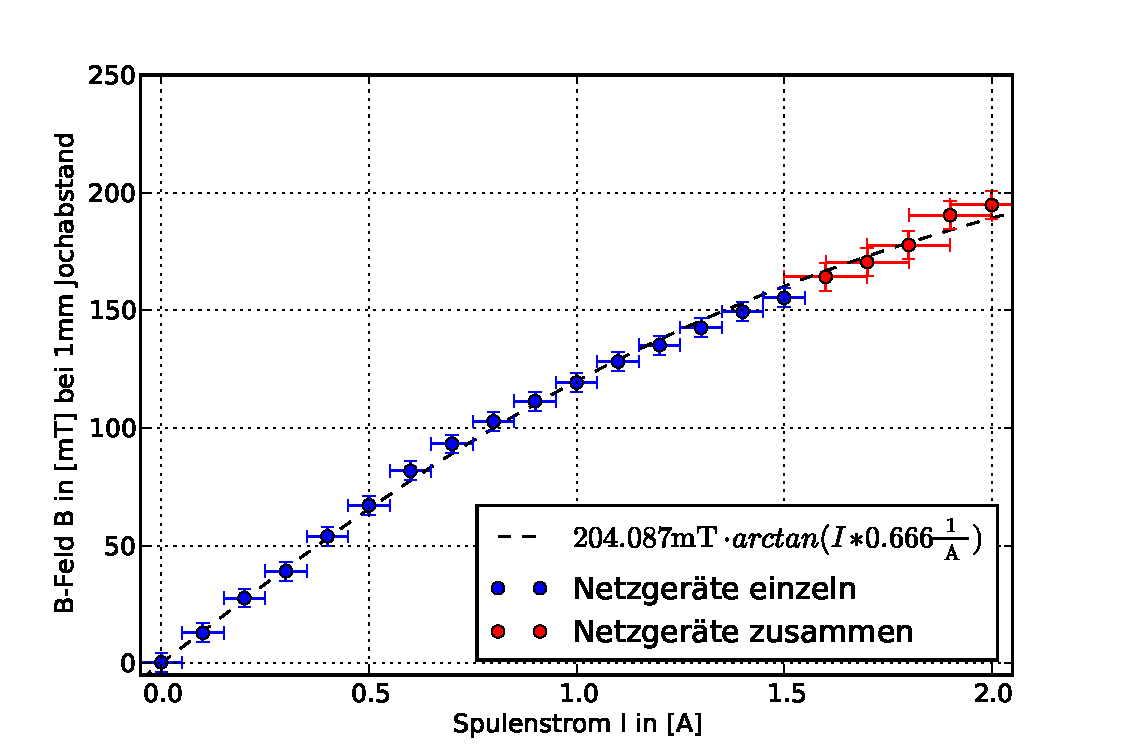
\includegraphics[width=0.8\textwidth]{images/messung_Strom-B-Feld.pdf}
\end{center}
\vspace{-1.5\baselineskip}
\caption{Abhängigkeit der Magnetfeldstärke von der an den vier Spulen angelegten Stromstärke}
\label{messung_Strom-B-Feld}
\end{figure}


\subsection{Aufbau der Zelle}			%%karl
Bei der Planung der Zellengeometrie mussten verschiedene Eigenschaften abgewägt werden, um eine möglichst hohe Leistung der Zelle zu erhalten.
Es gilt:
\begin{equation}
P \propto B^2 \cdot v^2 \cdot d \cdot A_{\text{Elektrode}}
\end{equation}
Wobei $B$ die Flussdichte des Magnetfeldes des Elektromagneten, $v$ die Durchflussgeschwindigkeit durch die Zelle, $d$ den Abstand der Elektroden und $A_{\text{Elektrode}}$ die Elektrodenfläche bezeichnen. 
Bei einer begrenzten Pumpenleistung und damit einem konstanten maximalen Volumendurchsatz $V=A_{\text{Durchfluss}} \cdot v=\text{const}$ ist die Geschwindigkeit $v$ indirekt proportional von der Durchflussfläche $A_{\text{Durchfluss}} = d \cdot b$ abhängig.
Die Breite $b$ der Zelle sollte klein gehalten werden, um ein möglichst starkes Magnetfeld zu gewährleisten. Deshalb wurde versucht eine hohe, schmale und dünnwandige Zelle zu konstruieren.
Unter Berücksichtigung der Geometrie des B-Feldes und mit Absprache der Werkstatt, ergab sich folgender Aufbau der Durchflusszelle:

\begin{figure}[ht]
\begin{center}
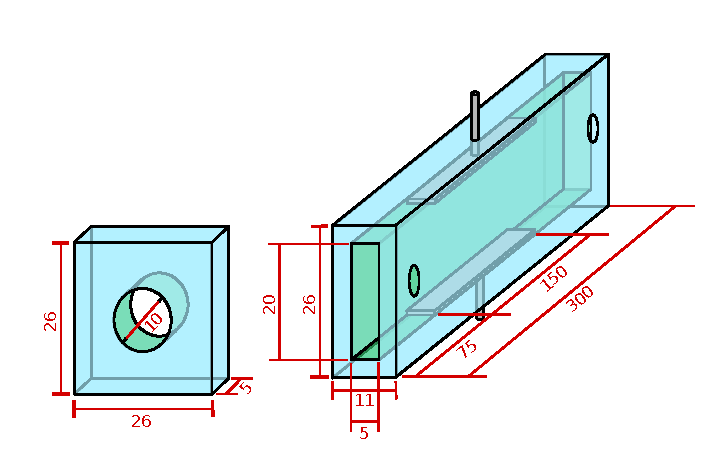
\includegraphics[width=0.8\textwidth]{images/zelle-schema.pdf}
\end{center}
\vspace{-1.5\baselineskip}
\caption{Schematischer Aufbau der Durchflusszelle (alle Angaben in mm)}
\label{zelle-schema}
\end{figure}

Als Elektrodenmaterial wurde zuerst Aluminium angedacht. Erste Versuche zeigten jedoch starke chemische Reaktionen mit der Salzwasserlösung, weshalb die Elektroden dann aus Edelstahl gefertigt wurden. 
An den in \abb{zelle-einzeln} zu erkennenden Löchern wurden Schlauchstutzen aus Kunststoff angebracht, um vorne und hinten den Durchlaufschlauch und seitlich dünnere Schläuche zur Druckmessung befestigen zu können.
Die mechanische Werkstatt fertigte zwei Durchflusszellen aus Plexiglas, die jedoch leider beide nicht wasserdicht waren. Mit Hilfe von Silikon konnten die Leckstellen abgedichtet werden.

\begin{figure}[ht]
\begin{center}
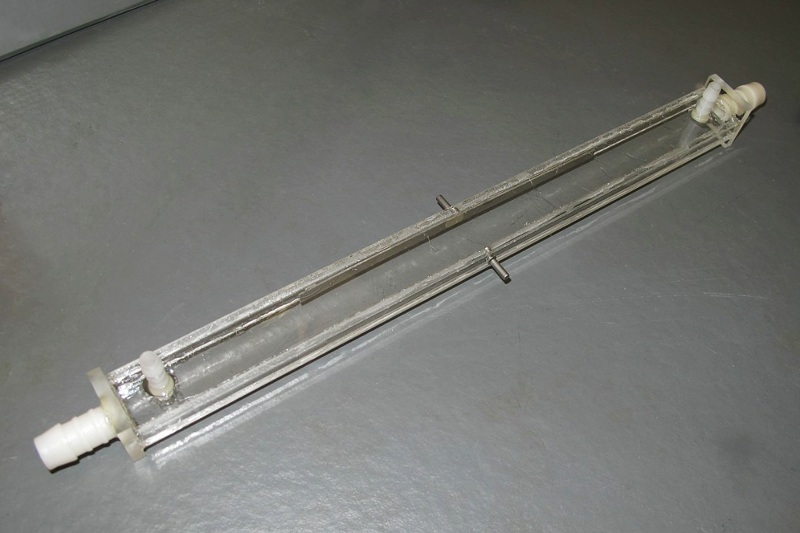
\includegraphics[width=1.0\textwidth]{images/zelle-einzeln.jpg}
\end{center}
\vspace{-1.5\baselineskip}
\caption{Die fertige Durchflusszelle mit Elektroden. Die seitlichen Stutzen dienen der Druckmessung.}
\label{zelle-einzeln}
\end{figure}

\subsection{Aufbau der Messapperatur}		%% Axi
Nachdem die Zelle in der Werkstatt fertiggestellt worden war, wurde die restliche Versuchanordnung aufgebaut. Der MHD-Generator sollte folgende Komponenten enthalten:

\begin{itemize}
	\item Eine Pumpe mit einem Reservoir an ges\"attigtem Salzwasser 
	\item die Zelle, platziert in einem m\"oglichst homogenen Magnetfeld 	
	\item M\"oglichkeiten zur Messung der Magnetfeldst\"arke sowie des lokalen Drucks in der Zelle.
\end{itemize}

Die Pumpe wurde bereits im Vorraus im Versandhandel bestellt. Die ersten Vorabrechnungen hatten ergaben, dass eine Wassergeschwindigkeit im Bereich von $1m/s$ messbare Ergebnisse liefern w\"urde. Daher entschieden wir uns f\"ur eine Teichpumpe, die mit 220V Netzspannung betrieben wird und dabei laut Herstellerangaben bei einer Leistung von 16W ca. $1000\unit{\ell}$ Wasser pro Stunde bis zu einer F\"orderh\"ohe von 1,7m transportieren soll. Da davon auszugehen war, dass diese nicht f\"ur den Einsatz in hoch konzentriertem Salzwasser geeignet ist, wurde der komplette Kreislauf am Ende jedes Arbeitstages mit Leitungswasser gesp\"ult um Langzeitsch\"aden vorzubeugen.

Beim Aufbau der gesamten Apperatur des MHD-Geneators musste mehreren Faktoren besondere Aufmerksamkeit geschenkt werden: 
\begin{itemize}
	\item Die Bereiche mit anliegenden Spannungen sollten getrennt von den wasserf\"uhrenden Bauteilen installiert werden. 
	\item Der Zelle muss waagrecht eingebaut sein, damit die Druckmessung nicht beeinflusst wird.
	\item Der Aufbau sollte genau reproduzierbar sein, um eine Vergleichbarkeit der Messungen zu erreichen.
	\item Bei einem Durchlauf sollten m\"oglichst viele Parameter gleichzeitig erfasst werden k\"onnen.
\end{itemize} 

\begin{figure}[ht]
\begin{center}
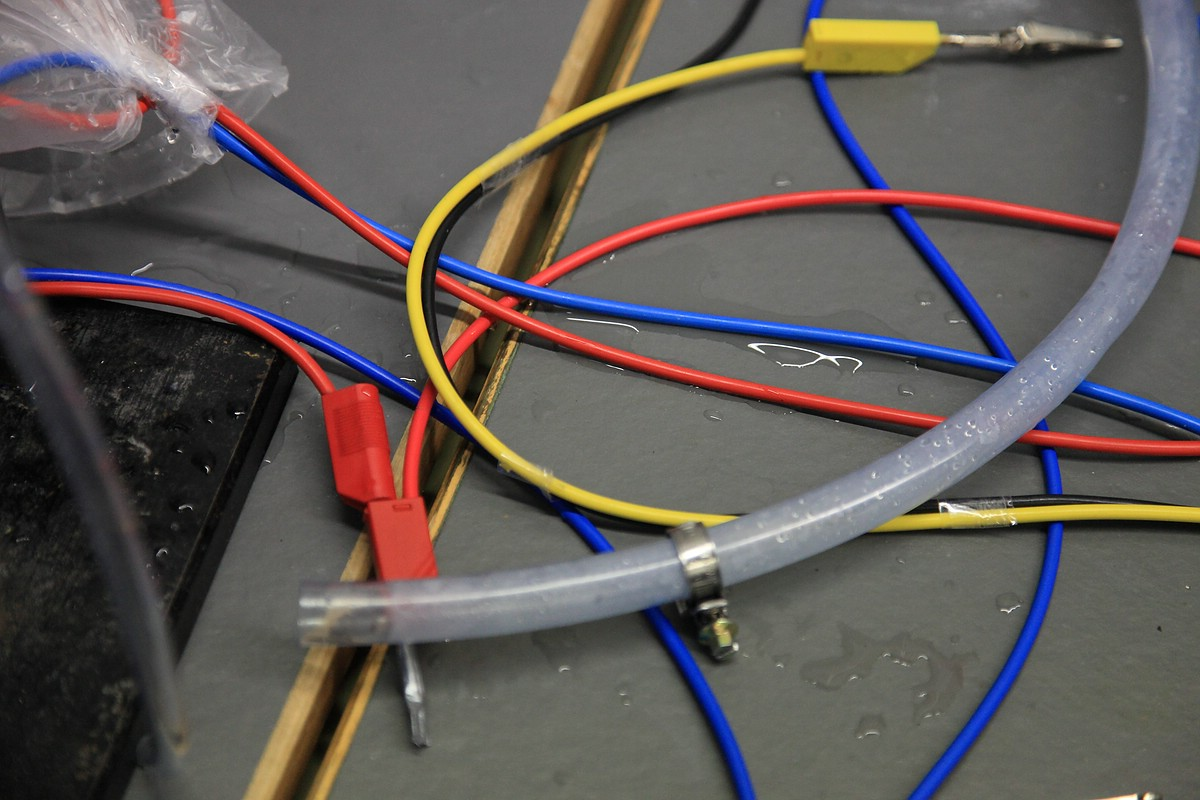
\includegraphics[width=0.8\textwidth]{images/wasser-strom1.jpg}
\end{center}
\vspace{-1.5\baselineskip}
\caption{Trennung der wasser- und stromf\"uhrenden Bereiche}
\label{wasser-strom1}
\end{figure}

Wie bereits beim ersten Projekt, erschien auch hier eine Konstruktion aus Stativstangen am Sinnvollsten. Die Zelle wurde an einem quadratischen Rahmen aus Stangen, Winkelverschraubungen, sowie Klemmen fixiert und konnte von oben in das Magnetfeld gesenkt werden. So war auch ein Umbau bei Bedarf relativ einfach m\"oglich. Eine vollst\"andige Trennung der strom- und wasserf\"uhrenden Teile ist aufgrund des MHD-Prinzips nicht m\"oglich. Daher befanden sich die Spulen und Eisenkerne mit den Stromanschl\"ussen in einer Plastikh\"ulle, die gen\"ugend Spielraum bot, um zwischen den Kernen die Zelle zu fixieren. 

Nachdem bei ersten Vormessungen entweder die Zelle oder die Magnetfeldsonde zwischen den  Spulen plaziert waren, entschieden wir uns auch die tangentiale B-Feld Sonde dauerhaft in den Kreislauf zu integrieren, um die Messwerte zusammenh\"angend aufzuzeichnen. Zwei d\"unne Abstandshalter stellten dabei sicher, dass die empfindliche Sonde nicht zwischen den Magneten zerdr\"uckt wird.

\begin{figure}[ht]
\begin{center}
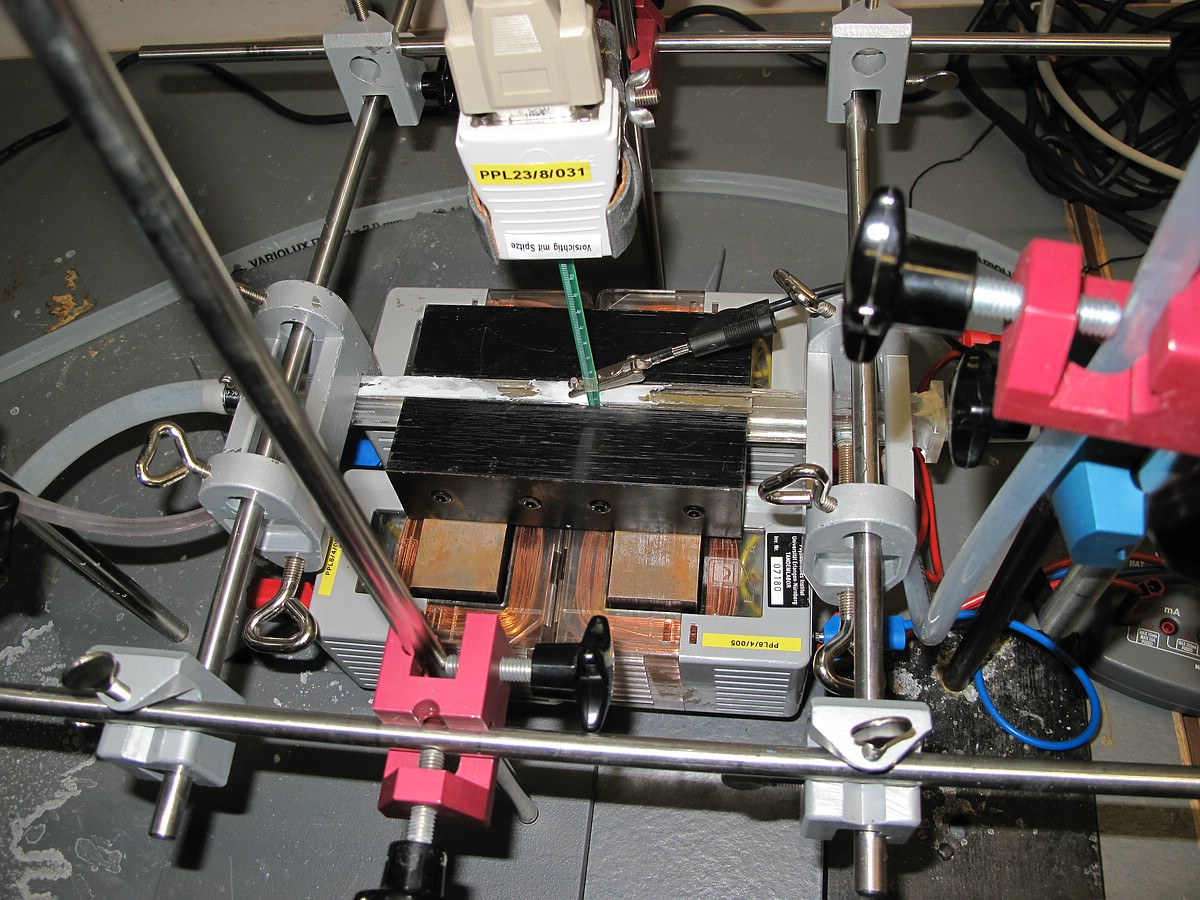
\includegraphics[width=0.8\textwidth]{images/offen.jpg}
\end{center}
\vspace{-1.5\baselineskip}
\caption{Die Magnetfeldsonde, eingeklemmt zwischen Spulenkernen und Zelle. Die Plastikt\"ute um die Spulen wurde aus optischen Gr\"unden entfernt.}
\label{offen}
\end{figure}

Zur Bestimmung des lokalen Drucks, kamen zwei d\"unne Schl\"auche als Steigrohre zum Einsatz, welche an den Seitenr\"andern der Zelle angeschlossen waren. An diesen konnte der unterschiedliche Wasserstand abgelesen werden. Um eine einheitliche Ausgangsh"ohe zu erhalten, kam als als Messbasis eine Wasserwaage zum Einsatz. Die Steigrohre wurden ebenfalls in die Konstruktion eingespannt.

\begin{figure}[ht]
\begin{center}
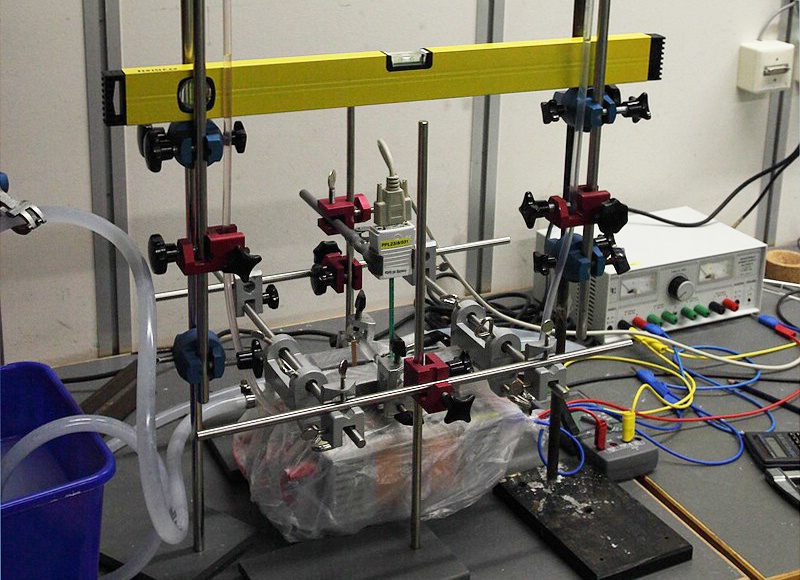
\includegraphics[width=0.8\textwidth]{images/wwaage.jpg}
\end{center}
\vspace{-1.5\baselineskip}
\caption{Der komplette Aufbau des MHD-Generators, im Eimer links befindet sich die Pumpe mit dem Wasservorrat}
\label{wwaage}
\end{figure}

Strom und Spannungsmesswerte, sowie die Magnetfeldst"arke wurden durch das Cassy Lab System mit entsprechenden Verst"arker und Anschlussboxen \"uber die Zeit aufgetragen und zur Auswertung aufgezeichnet. F\"ur die Messung des, an der Spule angelegten, Stroms im Bereich von bis zu $2A$, war der Messbereich ausreichend, es waren jedoch keine Adapter verf\"ugbar, um den an der Zelle abfallenden Strom zu verst\"arken. Daher kam auch hier wieder der Umweg \"uber einen einstellbaren Widerstand mit anschlie\"ssender Spannungsmessung zum Zuge.





\section{Messungen und Ergebnisse}

\subsection{Leitfähigkeit von Salzwasser}\label{leit}		%%michele - done
Um die Größenordnung der Leistung des MHD-Generators abschätzen zu können, ist es zunächst besonders wichtig den Leitwert von Salzwasser zu kennen.

\subsubsection{Vormessungen}
In einer ersten Vormessung wurden hierfür in einem mit Salzwasser gefüllten, quaderförmigen Bassin mit den Maßen $14.3 \unit{cm} \times 14.3 \unit{cm} \times 1.4 \unit{cm}$ Aluminuimelektroden an zwei entgegengesetzte Stirnflächen angebracht.
% evtl Foto ?
An diesen Elektroden wurde eine variable Spannung angelegt und der resultierende Strom aufgezeichnet. Die durch ein strakes Schwanken der Spannungswerte um bis zu $\pm 30 \unit{mV}$ erschwerte Messung wurde anschleißend für veschiedene Salzkonzentrationen wiederholt (siehe Abbildung \ref{widerstand_vormessung}).


\begin{figure}[ht]
\begin{center}
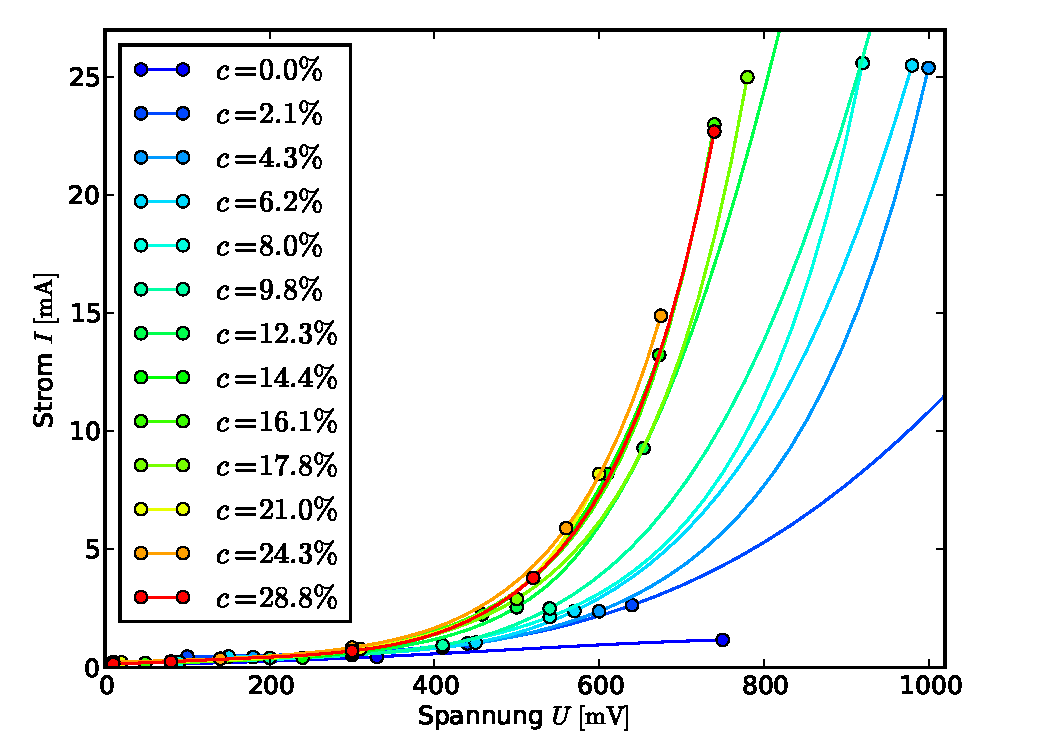
\includegraphics[width=1.0\textwidth]{images/kennlinien_lin.pdf}
\end{center}
\vspace{-1.5\baselineskip}
\caption{Widerstand von Salzwasser bei verschieden Konzentrationen}
\label{widerstand_vormessung}
\end{figure}

Deutlich zu erkennen ist der erwartete Zusammenhang zwischen Leitwert und Salzkonzentration. Der Widerstand liegt jeweils in der Größenordnung von $1\ee{1} \ \Omega$, der spezifische Widerstand somit im Bereich von $1 \ee{0} \ \Omega\unit{m}$. Leider sind die Ergebnisse der Messungen aufgrund der Unregelmäßigkeiten nicht besonders signifikant, sodass jeweils nur über die Größenordnung der Messwerte eine Aussage getroffen werden kann.

Diese Vormessung wurde nochmal nach dem Vier-Punkt-Messverfahren wiederholt, welches sicherstellt, dass die Fehler der Kontaktwiderstände an den Klemmen elimiert werden. Bei diesem Verfahren wird die Spannungsmessung über separate, nicht stromführende Kontakte ausgeführt, um Übergangswiderstände zu minimieren. Zudem konnten dank unseres Betreuers Messapparaturen aus dem Labor des Physikalischen Instituts III verwendet werden.
Bei den nun eingesetzten Kupferelektroden zeigte sich ein deutlich nicht-ohmscher Widerstand, bei Variation der Spannung ergab sich ein nichtlinearer und nichteinmal monotoner Stromverlauf, sondern nur eine Art unsaubere Hysterese. Mit den Aluminumelektroden aus der ersten Vormessung hatten wir ein ähnliches Ergebnis. Deutlich sauberer allerdings war die Kennlinien mit Edelstahlelektroden, trotzdem war immernoch eine verkleinerte und monotene Hystereseform erkennbar. Die Ursache für diese Nichtlinearität sehen wir in elektrochemischen Prozessen, da sie offensichtlich vom verwendeten Elektrodenmaterial abhängig ist. Aufgrund dieser Ergebnisse entschieden wir uns dafür auch bei unserer finalen Zelle Edelstahlelektroden zu verwenden.

Der spezifische Widerstand konnte bei dieser zweiten Vormessung auf einen Bereich von $1 \ee{2} \ \Omega \unit{m}$ abgeschätzt werden, bei einer Salzkonzentration von $15 \%$

\subsubsection{Messung an der Zelle}
Um schließlich einen für unseren endgültigen Messaufbau validen Widerstandswert zu erhalten, führten wir die Messungen nochmal an der eigentlich verwendeten Zelle durch. Es wurde wieder nach dem Vier-Punkt-Verfahren gemessen, nun allerdings nicht mehr mit den professionellen Messgeräten sondern mit dem Cassy-System. Im Messprozess wurde ein bekannter Strom in der Größenordnung des eigentlich zu messenden MHD-Effekts an die Zelle angelegt und die resultierende Spannung aufgezeichnet, das Ergebnis ist die $I$-$U$-Kennlinie in Abbildung \ref{widerstand_zelle}. Diese setzt sich zusammen aus einem Bereich mit ansteigenden Strom (unten) sowie mit absinkenden Strom (oben). Zudem zeigt sich ein weiterer Effekt: selbst bei konstantem Strom driftet die gemessene Spannung mit einer Rate von $\frac{\dif U}{\dif t} = 0.415 \frac{\unit{mV}}{\unit{s}}$ (rechts) bzw. $\frac{\dif U}{\dif t} = -0.274 \frac{\unit{mV}}{\unit{s}}$ (links) (jeder der vier Bereiche wurde in einer Zeitspanne von $30\ldots40 \unit{s}$ aufgezeichnet).

\begin{figure}[ht]
\begin{center}
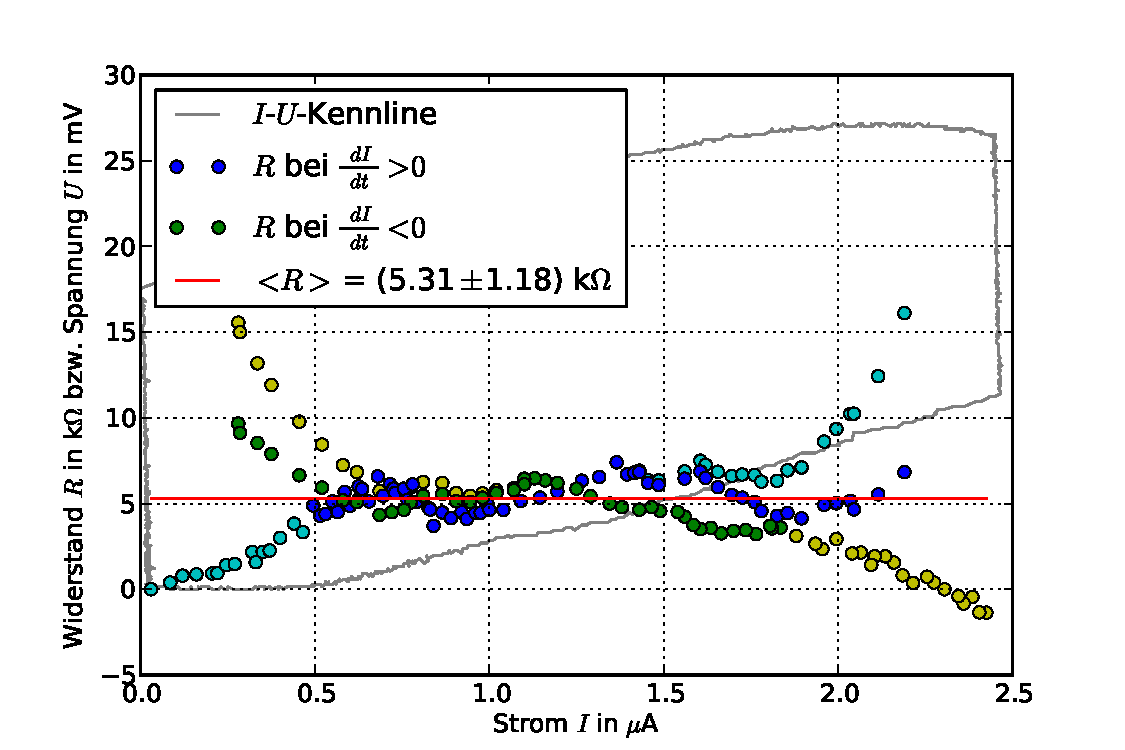
\includegraphics[width=1.0\textwidth]{images/messung_widerstand.pdf}
\end{center}
\vspace{-1.5\baselineskip}
\caption{Widerstandswert der verwendeten Zelle bei gesättigter Salzlösung}
\label{widerstand_zelle}
\end{figure}

Die aus der Messung erhaltenen Widerstandswerte finden sich ebenfalls in Abbildung \ref{widerstand_zelle}, wobei die steigende (hell-/blau) und fallende Flanke (hell-/grün) getrennt behandelt wurden, die später aus der Mittelwertbildung ausgeschlossenen Werte sind in einem helleren Farbton gezeichnet. Man erkannt dank der Symmetrie der beiden Kurven, dass, zumindest in der Größenordnung vom $\unit{\mu A}$, keine Abhängigkeit des Widerstands von Strom vorliegt, sondern vielmehr von elektrochemischen Prozessen bei Herauf- und Herabfahren der Stromstärke.
Die Überhöhungen der Widerstandswerte bis hin zu $15 \unit{k}\Omega$ können mit den erwähnten Spannungsdriften  erklärt und korrigiert werden. Hierfür wurde ein linearer Anstieg dieser Driftraten mit dem Strom im Bereich des steilen Widerstandsanstieges ($1.5\ldots2.45 \unit{\mu A}$ für den ansteigenden bzw. $0.0\ldots1.0 \unit{\mu A}$ für den abfallenden Strombereich) angenommen. Für die übertrieben kleinen bis hin zu negativen Widerstandswerte (vgl. auch die horizintalen Abschnitte der Kennlinie) kann allerdings keine befriedigende Erklärung gefunden werden, weshalb diese Bereich einfach von der Mittelwertbildung ausgeschlossen werden. Auf diesem Weg erhalten wir schließlich einen Wert von
\begin{equation}
R = (5.31 \pm 1.18) \, \unit{k}\Omega
\end{equation}
für unsere finale Zelle bei einer gesättigen Salzlösung.


\subsection{Magnetfeld}		 	%%andi
Eine weiterer Messung zielte auf die Ermittlung der Abhängigkeit der Zellspannung vom angelegten Magnetfeld hin. Theoretisch müsste sich nach
\begin{equation}
U = B \cdot v \cdot d,
\end{equation}
eine lineare Abhängigkeit ergeben (für $B,v=const$). Eine erste Messreihe, bei der die beiden für diese Messung unerheblichen Druckmessungsschläuche (siehe \hyperref[wwaage]{Abb.~\ref{wwaage}}) per Hand verschlossen wurde, lieferte scheinbare willkürliche Werte für die Zellspannung. Nach einer Befestigung dieser Schläuche lieferte der Aufbau jedoch Werte, die einwandfrei mit der Theorie übereinstimmten (siehe \hyperref[spannung]{Abb.~\ref{spannung}}). \

\begin{figure}[ht]
\begin{center}
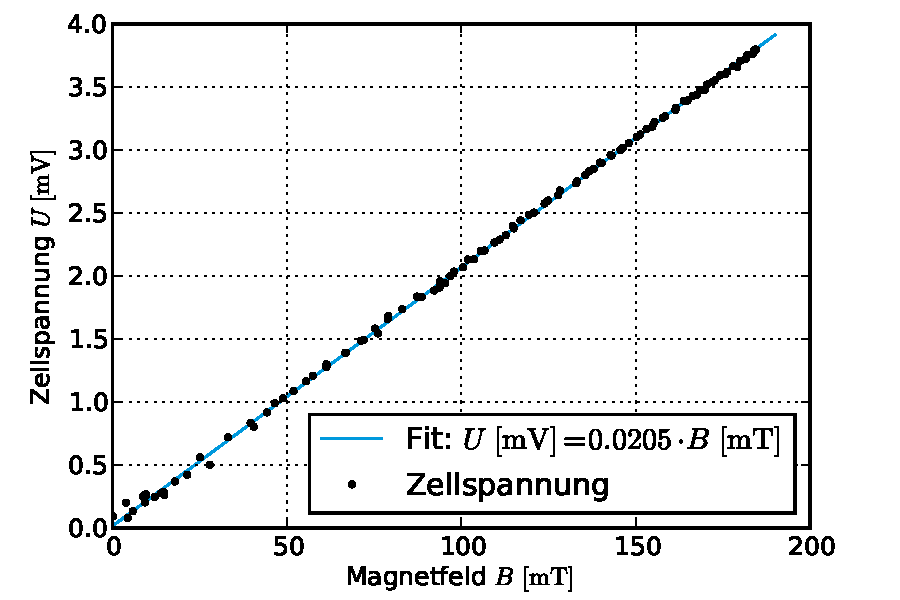
\includegraphics[width=1.0\textwidth]{images/spannung.pdf}
\end{center}
\vspace{-1.5\baselineskip}
\caption{Zellspannungswerte in Abhängigkeit von der Magnetfeldstärke}
\label{spannung}
\end{figure}

\hyperref[messkurve_spannung]{Abb.~\ref{messkurve_spannung}} zeigt exemplarisch den Zellspannungsverlauf für beim Auf-bzw Abbau des angelegten Magnetfeldes (Peak-Wert $B \approx 280 \unit{mT}$). Auch hier ist gut erkennbar, dass $U \propto B$ gilt. \
Zu beachten war bei der Spannungsmessung, dass eine Grundspannung $U_0$ (siehe \hyperref[messkurve_spannung]{Abb.~\ref{messkurve_spannung}}) an den Elektroden auch dann zu beobachten war, wenn kein Magnetfeld angelegt wurde. Diese Grundspannung reduzierte anfangs in etwa exponentiell, dann näherte sie sich asymptotisch an die Nullspannung an. Bis zum Redaktionsschluss konnte trotz großer Bemühungen keine Erklärung für diese Grundspannung gefunden werden.  


\begin{figure}[ht]
\begin{center}
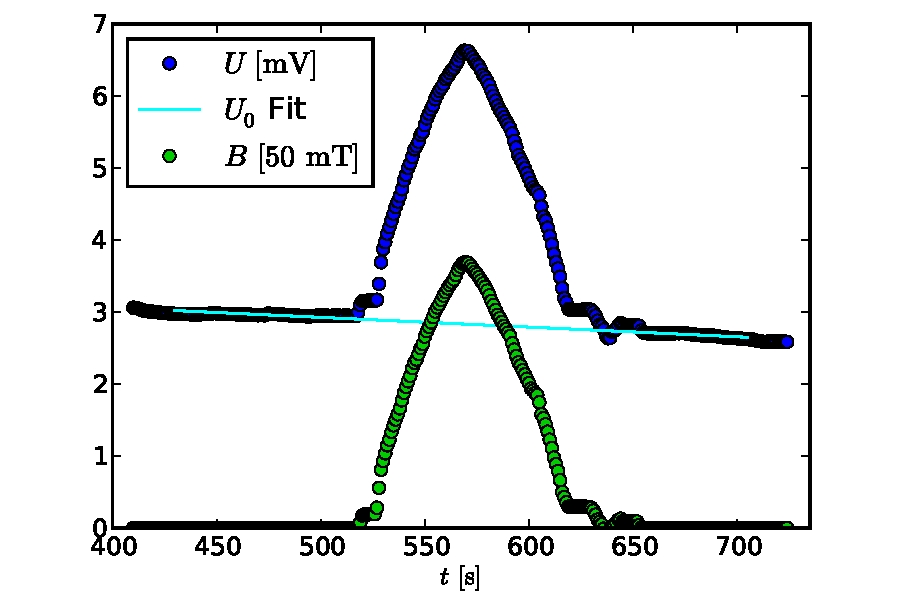
\includegraphics[width=1.0\textwidth]{images/messkurve_spannung.pdf}
\end{center}
\vspace{-1.5\baselineskip}
\caption{Spannungswerte am Außenwiderstand in Abhängigkeit vom Widerstand und dem Magnetfeld}
\label{messkurve_spannung}
\end{figure}


\subsection{Zellspannung und -strom}		%%basti
\begin{figure}[ht]
\begin{center}
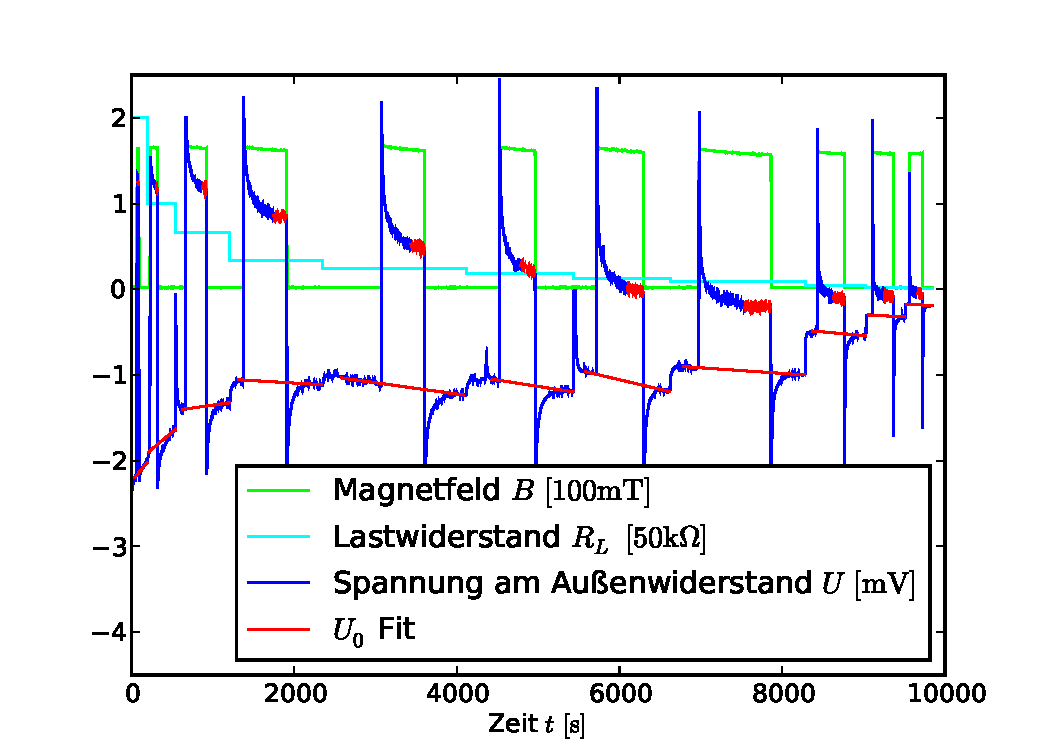
\includegraphics[width=1.0\textwidth]{images/rohdaten_strom.pdf}
\end{center}
\vspace{-1.5\baselineskip}
\caption{Spannungswerte am Außenwiderstand in Abhängigkeit vom Widerstand und dem Magnetfeld}
\label{rohdatenstrom}
\end{figure}
Prinzipiell dient ein Generator dazu, elektrische Leistung zu erzeugen, und das kann er nur wenn mit der induzierten Spannung ein Strom fließt.
Wie es sich gezeigt hat, erhalten wir bei der verwendeten Fließgeschwindigkeit von $v=1,4\unit{\frac{m}{s}}$ leider nur Ströme im $\mathrm{\mu A}$-Bereich.
Deshalb wäre die Messung über ein Amperemeter recht schwierig gewesen und wir haben uns für eine indirekte Methode entschieden.

Das verwendete Voltmeter des Cassy-systems besitzt einen Innenwiderstand von $R_{\text{U}} = 100\unit{k\Omega}$.
Sein Stromfluss ergibt sich ganz einfach nach dem ohmschen Gesetz.
Zusätzlich wurden nun verschiedene Lastwiderstände $R_{\text{L}}$ parallel geschalten und der Gesamtstrom in der Schaltung bzw. Zelle ist folglich
\begin{equation}
I
= \frac{U}{R}
= \frac{U}{(R_{\text{U}}^{-1} + R_{\text{L}}^{-1})^{-1}}
= U\cdot\left(\frac{1}{R_{\text{U}}} + \frac{1}{R_{\text{L}}}\right)
\label{stromrechnung}
\end{equation}
\begin{table}[ht]
\captionabove{Ausgewertete Spannungs- und Stromwerte bei $B = 160\unit{mT}$}
\label{tab:strom}
\begin{center}\vspace{-\baselineskip}
\begin{tabular}{rr|cc}
$R_{\text{L}} \; \unit{[k\Omega]}$ &
$R \; \unit{[k\Omega]}$ &
$U\; \unit{[mV]}$ &
$I\; \unit{[\mu A]}$ \\
\hline
$\infty$ & 100,00 & 3,16 & 0,032 \\
100 & 50,00 & 2,79 & 0,056 \\
50 & 33,33 & 2,51 & 0,075 \\
20 & 16,67 & 1,93 & 0,116 \\
14 & 12,28 & 1,65 & 0,134 \\
10 & 9,09 & 1,35 & 0,149 \\
7 & 6,54 & 1,10 & 0,168 \\
5 & 4,76 & 0,78 & 0,164 \\
2 & 1,96 & 0,42 & 0,215 \\
1 & 0,99 & 0,24 & 0,244 \\
0,5 & 0,50 & 0,14 & 0,275
\end{tabular}
\vspace{-\baselineskip}\end{center}
\end{table}

Die Apperatur zeigte bei der Messung wieder eine zeitabhängige Offsetspannung in der gleichen Größenordnung des Signals, welche daher unbedingt zu eliminieren war.
Hierzu wurde jeweils der gewünschte Lastwiderstand angeklemmt, dann ein stabiler Spannungsverlauf abgewartet.
Sobald dieser vorhanden war, wurde das Magnetfeld aktiviert und wieder gewartet.
Hier konnte es schon 10 Minuten dauern, bis das Signal asymptotisch wurde.
Daraufhin wurde das Magnetfeld wieder deaktiviert und ein letztes mal gewartet.
In \abb{rohdatenstrom} ist der resultierende Spannungsverlauf dargestellt.
Die Offsetspannung konnte nun (als rote Linien dargestellt) in den Graphen gefittet und die Differenzen zu den höheren Spannungswerten gemessen werden.
Die Spannungswerte wurden punktweise durch das vorherrschende -- nicht ganz konstante -- Magnetfeld geteilt und dann für jeden Widerstandswert gemittelt.
Die Ausgabe des hierzu erstellten Pythonprogramms findet sich in \tab{tab:strom}, wobei die Strom- und spannungswerte wieder mit der mittleren Flussdichte von $160\unit{mT}$ hochgerechnet sind.

Die so ermittelten Spannungs- und Stromwerte sind in \abb{fig:strom} aufgetragen.
Aus den Daten errechnet sich nun, dass die Zellspannung unter gegebenen Umständen bei $U = (3,7 \pm 0,2)\unit{mV}$ lag und der Eigenwiderstand der Zelle in diesem Spannungsbereich bei
\begin{equation}
R_{\text{Z}} = (15,7 \pm 1,7)\unit{k\Omega}
\end{equation}
mit einer Kovarianz der beiden Werte von $0,33\unit{mV}\unit{k\Omega}$.
Einen derart hohen Widerstandswert hatten wir nicht erwartet.
Bei unserer Zellgeometrie von $1,8\unit{cm}\times 7,5\unit{cm^2}$ ergibt dies einen Leitwert von
\begin{equation}
\sigma
= \frac{d}{R\,A}
= (0,001\,53 \pm 0,000\,17)\ee{-3}\unit{\frac{1}{\Omega m}}
\qquad
\text{ bei } U\approx 3\unit{mV}
\label{eqn:sigma}
\end{equation}
Dies ist erstaunlich wenig, wenn man bedenkt dass der Leitwert von Leitungswasser in etwa bei $0,05\unit{\Omega^{-1}m^{-1}}$ und von Salzwasser sogar bei $5\unit{\Omega^{-1}m^{-1}}$ liegen sollte.
Das Ergebnis geht also konform mit unseren anderen Erkenntnissen zur Leitfähigkeit von Salzwasser, dass diese für geringe Gleichspannungen deutlich verringert ist.

\begin{figure}[H]
\begin{center}
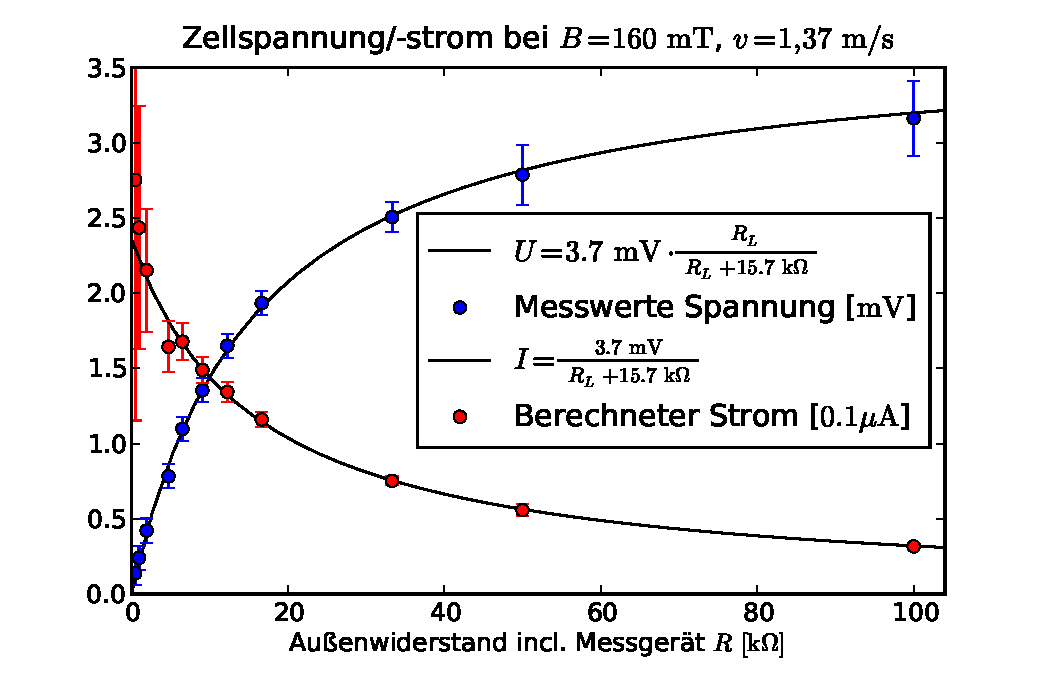
\includegraphics[width=1.0\textwidth]{images/strom.pdf}
\end{center}
\vspace{-1.5\baselineskip}
\caption{Spannung und Strom an der Zelle}
\label{fig:strom}
\end{figure}

Für unseren MHD-Generator bedeutet das konsequenterweise, dass mit den gegebenen Parametern keine sinnvolle Stromerzeugung möglich ist. Wie im \hyperref[leit]{Abschnitt~\ref{leit}} festgestellt wären dazu Spannungen in der Größenordnung ab $1\unit{V}$ notwendig, wozu man das Produkt aus Magnetfeld, Elektrodenabstand und Fließgeschwindigkeit um den Faktor 300 erhöhen müsste. Das ist großtechnisch wohl machbar, liegt aber außerhalb unserer Verbesserungsmöglichkeiten.




\subsection{Wassergeschwindigkeit und Druck}		%%karl 
Zur Bestimmung des Wirkungsgrads des MHD-Generators wäre eine Druckdifferenzmessung vor und hinter den Elektroden nötig gewesen.
Es wurde versucht dies mit Hilfe der Steighöhe in den beiden seitlich angebrachten Schläuchen zu bestimmen. Leider waren die Schwankungen im Pumpbetrieb wesentlich stärker als der zu messende Steighöhenunterschied.
Eine Wirkungsgradbestimmung war somit unmöglich.

Zur Bestimmung der Abhängigkeit der generierten Spannung von der Durchflussgeschwindigkeit durch die Zelle, musste ein Weg gefunden werden die Pumpe, die eigentlich einen konstanten Fluss lieferte zu drosseln.
Ein mitgeliefertes Ventil konnte verwendet werden, um den Volumendurchsatz der Pumpe zu reduzieren. So war es möglich verschiedene Geschwindigkeiten durch die Zelle zu realisieren.
Um den Betrag der Durchflussgeschwindigkeit zu ermitteln wurde die Zeit $t$ genommen, die die Pumpe benötigte um ein konstantes Volumen $V=400\unit{ml}$ mit Wasser zu füllen. Um statistische Fehler zu minimieren wurde dies bei eingestelltem Ventil mehrmals durchgeführt und über die Zeitwerte gemittelt.
Mit Hilfe des Volumendurchsatzes konnte dann die Durchflussgeschwindigkeit $v$ in der Zelle mit Querschnitt $A_{\text{Durchfluss}}$ ermittelt werden:
\begin{equation}
v=\frac{\text{Volumendurchsatz pro Zeit}}{A_{\text{Durchfluss}}}
\end{equation}
Der Querschnitt der verwendeten Zelle betrug $A_{\text{Durchfluss}}=0,5\unit{cm} \cdot 1,8\unit{cm}=0,9\unit{cm^{2}}$.

Die Unsicherheit der Geschwindigkeit ist durch das manuelle Stoppen der Zeitwerte bedingt und wird auf etwa $\Delta v=7\% \cdot v$ geschätzt.
Natürlich wird die Durchflussgeschwindigkeit innerhalb der Zelle eigentlich durch eine parabelförmige Geschwindigkeitsverteilung beschrieben, die aber hier in guter Näherung als konstant angenommen wird. 

Für die verschiedenen Durchflussgeschwindigkeiten konnte mit Hilfe des Cassy Lab Systems Spannung und B-Feld über die Zeit gemessen werden. Es wurde darauf geachtet, dass sich die Spannungskurve bereits 'eingependelt' hatte, um keine Störung durch die elektrochemischen und kapazitiven (???) Prozesse zu messen.
Bei jeder Geschwindigkeit wurde die Referenzspannung, d.h. die Spannung bei ausgeschaltetem B-Feld (nur Restmagnetisierung des Eisenjochs) gemessen und dann mehrmals das Magnetfeld ein- und ausgeschaltet.
Folgender Verlauf wurde beispielsweise für $v=0,68\frac{\unit{m}}{\unit{s}}$ aufgezeichnet:

%%Ich will das Diagramm genau hier haben! Geht das? Notfalls kleiner? -> ja, benutze ein [H]! Kann man das Bild nicht auch per Verweis referenzieren?

\begin{figure}[H]
\begin{center}
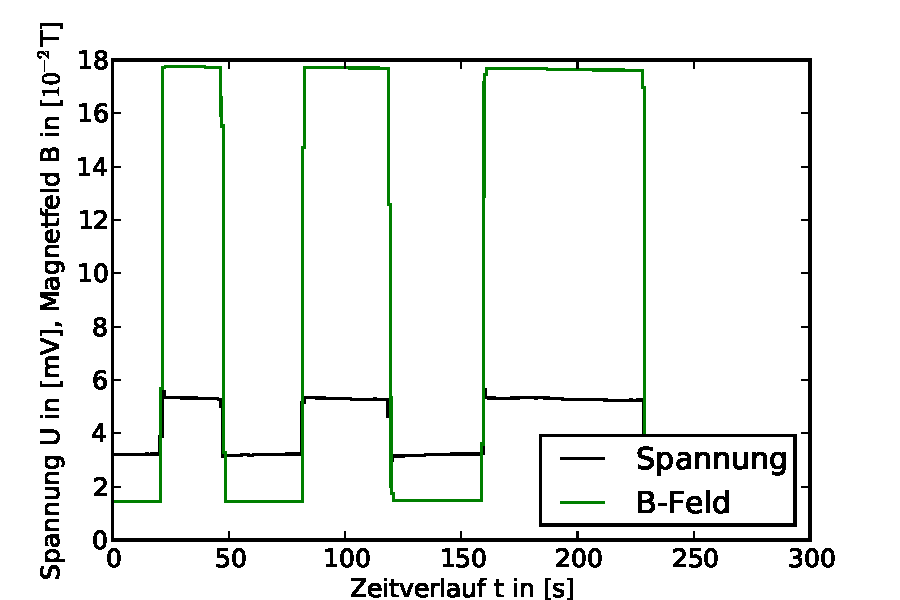
\includegraphics[width=0.8\textwidth]{images/U-B-068.pdf}
\end{center}
\vspace{-1.5\baselineskip}
\caption{Spannungs- und B-Feld-Verlauf für $v=0,68\frac{\unit{m}}{\unit{s}}$}
\label{U-B-068}
\end{figure}

Aus diesen Daten konnte für jede Geschwindigkeit der Spannungsunterschied und der Anstieg des B-Feldes ermittelt werden. 

\begin{table}[ht]
\captionabove{Messwerte zur Geschwindigkeitsabhängigkeit der Spannung}
\label{Geschwindigkeitstabelle}
\begin{center}\vspace{-\baselineskip}
\begin{tabular}{c|c}
$v\; \unit{[\frac{m}{s}]}$ &
$\frac{\Delta U}{\Delta B}\; \unit{[\frac{mV}{T}]}$ \\
\hline
0,35	& 6,69 \\
0,48	& 8,98 \\
0,68	& 12,96 \\
0,80	& 15,11 \\
0,96	& 18,29
\end{tabular}
\vspace{-\baselineskip}\end{center}
\end{table}

Um Spannungswerte bei leicht verschiedenen Magnetfeldern (unterschiedliche Magnetisierung des Eisenjochs) vergleichen zu können, wurde der Quotient aus Spannung und B-Feld über der Durchflussgeschwindigkeit aufgetragen:

\begin{figure}[ht]
\begin{center}
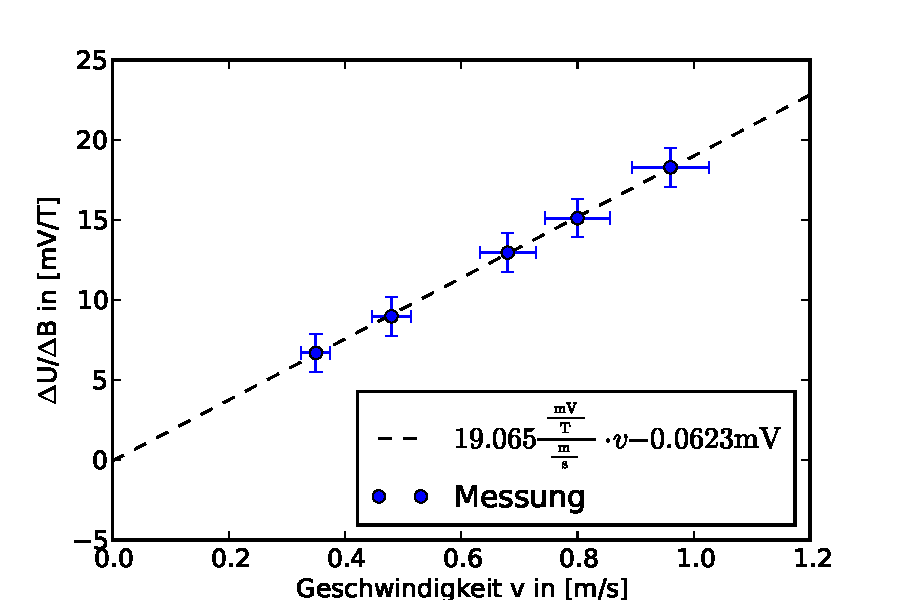
\includegraphics[width=0.8\textwidth]{images/v-U.pdf}
\end{center}
\vspace{-1.5\baselineskip}
\caption{Abhängigkeit von Durchflussgeschwindigkeit und generierter Spannung}
\label{v-U}
\end{figure}

Das theoretische Modell für die Spannung ergibt sich aus der Lorentzkraft für geladene Teilchen in einem homogenen Magnetfeld:
\begin{equation}
F=Q\cdot v\cdot B = Q \cdot E = Q \cdot \frac{U}{d}
\end{equation}
\begin{equation}
U=B \cdot d \cdot v
\end{equation}
\begin{equation}
\frac{\Delta U}{\Delta B}=d \cdot v
\end{equation}

Die lineare Abhängigkeit von Strom und Geschwindigkeit ist hervorragend erkennbar. Die Steigung der Fit-Geraden gibt laut Theorie den Abstand $d$ der Elektroden an. Sie beträgt $19 \unit{\frac{ mV/T }{ m/s }} = 19 \unit{mm}$ und stimmt damit sehr gut mit dem Abstand der Edelstahlplatten in unserer Zelle (18\unit{mm}) überein.


\subsection{Umkehrung des Effekts, Nutzung als Wasserpumpe}		%%david

Eine andere Nutzung des magentohydrodynamischen Effekts als die der Stromerzeugung entsteht dadurch, wenn man nun nicht fließendes Wasser benutzt, sondern bei Anwesenheit eines äußeren magnetischen Feldes Strom durch die Zelle schickt. Es ist somit quasi die Umkehrung des MHD-Generators und erzeugt einen Wasserfluss, welcher entweder als Antrieb oder Pumpe genutzt werden kann. So wurde in den 90er Jahren ein Schiff mit einem MH-Antrieb als Prototyp gebaut, welches allerdings aufgrund einiger Schwierigkeiten nicht über eine Geschwindigkeit von 15km/h hinaus kam.\footnote{\url{http://de.wikipedia.org/wiki/Magnetohydrodynamischer\_Antrieb}} Eine vielversprechendere Weiterführung des Gedankes ist der Magnetoplasmadynamische Antrieb, welcher nicht Wasser sondern Plasma als Medium benutzt und mit welchem bereits Austrittsgeschwindigkeiten des Plasmas von 40km/s erreicht wurden.\footnote{\url{http://de.wikipedia.org/wiki/Magnetoplasmadynamischer\_Antrieb}}

Bei der Durchführung unseres Versuches lösten wir den Schlauch von der Pumpe und legten beide Enden in den Wasserbehälter, um den Fließwiderstand durch die Pumpe hindurch zu eliminieren. Wir legten ein magnetisches Feld von $ B = (150 \pm 1) \unit{mT} $ an und schickten einen Strom von $I = (1,125 \pm 0,02) \unit{A}$ durch die Zelle. Die Dichte des Salzwassers wurde zuvor mithilfe einer Waage und eines Messbechers zu $\rho = (1,125 \pm 0,02) \unit{\frac{kg}{\ell}}$ bestimmt.\\
Es stellte sich jedoch heraus, dass man an den Enden der Schläuche keinen Wasserfluss spüren konnte, da der Fließwiderstand des Systemes anscheinend trotz Herausnahme der Pumpe noch zu groß war.

Um dennoch die theoretisch erreichbare Fließgeschwindigkeit des Wassers bestimmen zu können, wurden die beiden Schlauchenden verstopft, wodurch sich in den Steigrohren vor und nach den Elektroden der Zelle ein Pegelunterschied ergab. Dieser betrug $\Delta h = (2,8 \pm 0,2) \unit{mm}$. Zur Verifizierung, dass dies auch wirklich auf dem nachzuweisenden Effekt beruht, wurde die Stromrichtung umgekehrt, was zur Folge hatte, dass wieder der gleiche Pegelunterschied $\Delta h$ entstand, jedoch war nun, wie erhofft, der höhere Pegelstand in dem Steigrohr, in welchem zuvor noch der kleinere war.

Aus diesem Pegelunterschied lässt sich nun der Druckunterschied $\Delta p$ berechnen:
\begin{equation}
\Delta p = g \cdot \rho \cdot \Delta h = (31 \pm 2) \unit{Pa}
\end{equation}
Hierbei entspricht $g = 9,81 \unit{\frac{m}{s^2}}$ der Schwerebeschleunigung.\\
Nach dem Gesetz von Bernoulli
\begin{equation}\frac{1}{2}\cdot\rho\cdot v^2_{\text{Fluss}} + p = const
\end{equation}
kann man nun die nominelle Fließgeschwindigkeit berechnen und erhält
\begin{equation}
v_{\text{Fluss}} = (0,23 \pm 0,06)\unit{\frac{m}{s}}.
\end{equation}



\section{Fazit}		%%david

\newpage
\section{Autorenverzeichnis}
\begin{tabular}{|l|l|}
\hline
\emph{Autor} & \emph{Kapitel}\\
\hline
Michele Collodo & Widerstandsmessung\\
Andreas Glossner & Magnetfeldmessung\\
Karl-Christoph G\"odel & Bau der Zelle\\
Bastian Hacker & Strommessung\\
Maria Obst & Einleitung und Theorie\\
Alexander Wagner & Versuchsaufbau und Bilder\\
David Winnekens & Umkehrung des Effekts und Fazit\\
\hline
\end{tabular}

\end{document}
